\section{Statistical model of SER for MCP-PMT}\label{sec:model}
The MC calculation in Sec.~\ref{sec:convolution} can be expressed using mathematical equations
and abstracted into a model describing the charge of the MCP-PMT shown as Eq.~\eqref{eq:gammaTweedie}:
\begin{equation}
    \label{eq:gammaTweedie}
    \begin{aligned}
        Q_{\mathrm{MCP-PMT}} & = p\times Q_{\mathrm{channel}} + (1-p)\times Q_{\mathrm{surface}}                      \\
                             & = p\times Q_{\mathrm{channel}}+(1-p)\times (p_{\mathrm{ts}}
        \times Q_{\mathrm{ts}}+p_{\mathrm{rd}}\times Q_{\mathrm{rd}}+p_{\mathrm{bs}}\times Q_{\mathrm{bs}})           \\
                             & = p_0\times Q_{\mathrm{peak}} + (1-p_0)Q_{\mathrm{ts}}                                 \\
                             & = p_0\times Q_{\mathrm{peak}} + (1-p_0)\sum_{n=0}^{\infty}\sum_{i=0}^{n}Q_{\mathrm{i}}
    \end{aligned}
\end{equation}

In Eq.~\eqref{eq:gammaTweedie}, the spectra of $Q_{\mathrm{channel}}$, $Q_{\mathrm{rd}}$ and $Q_{\mathrm{bs}}$ are similar and
merged into a new component defined as $Q_{\mathrm{peak}}$ which follows Gamma distribution.
The other component is just $Q_{\mathrm{ts}}$ which is the reason
for the generation of the large charges in SER charge spectrum.

In MC calculation, $Q_{\mathrm{i}}$ follows Gamma distribution $\varGamma(\alpha_{\mathrm{i}},\beta_{\mathrm{i}})$ determined by $E_{\mathrm{i}}$,
the energy of true-secondary electrons which satisfies $\sum_i^nE_{\mathrm{i}}<E_0$.
Due to $n$ following the Poisson distribution with a mean between 5 and 7,
the probability of $n$ exceeding 10 is negligible.
At the same time, the total energy of the electrons is 650,
which is tens of times the energy of the true-secondary electrons in the SES.
The effect of $n$ on $E_{\mathrm{i}}$ can be ingnored
and all the energies of true-secondary electrons follow the same distribution.
As a result, the charge response of every true-secondary electron
can be treated indistinguishable regardless of the value of $n$ shown in Fig.~\ref{fig:single_pe}.
A Gamma distribution is deployed to fit the charge response of single true-secondary electron
shown in Fig.~\ref{fig:single_fit} and obtains a sufficiently good fit.

\begin{figure}[ht]
    \centering
    \begin{subfigure}{0.45\textwidth}
        \centering
        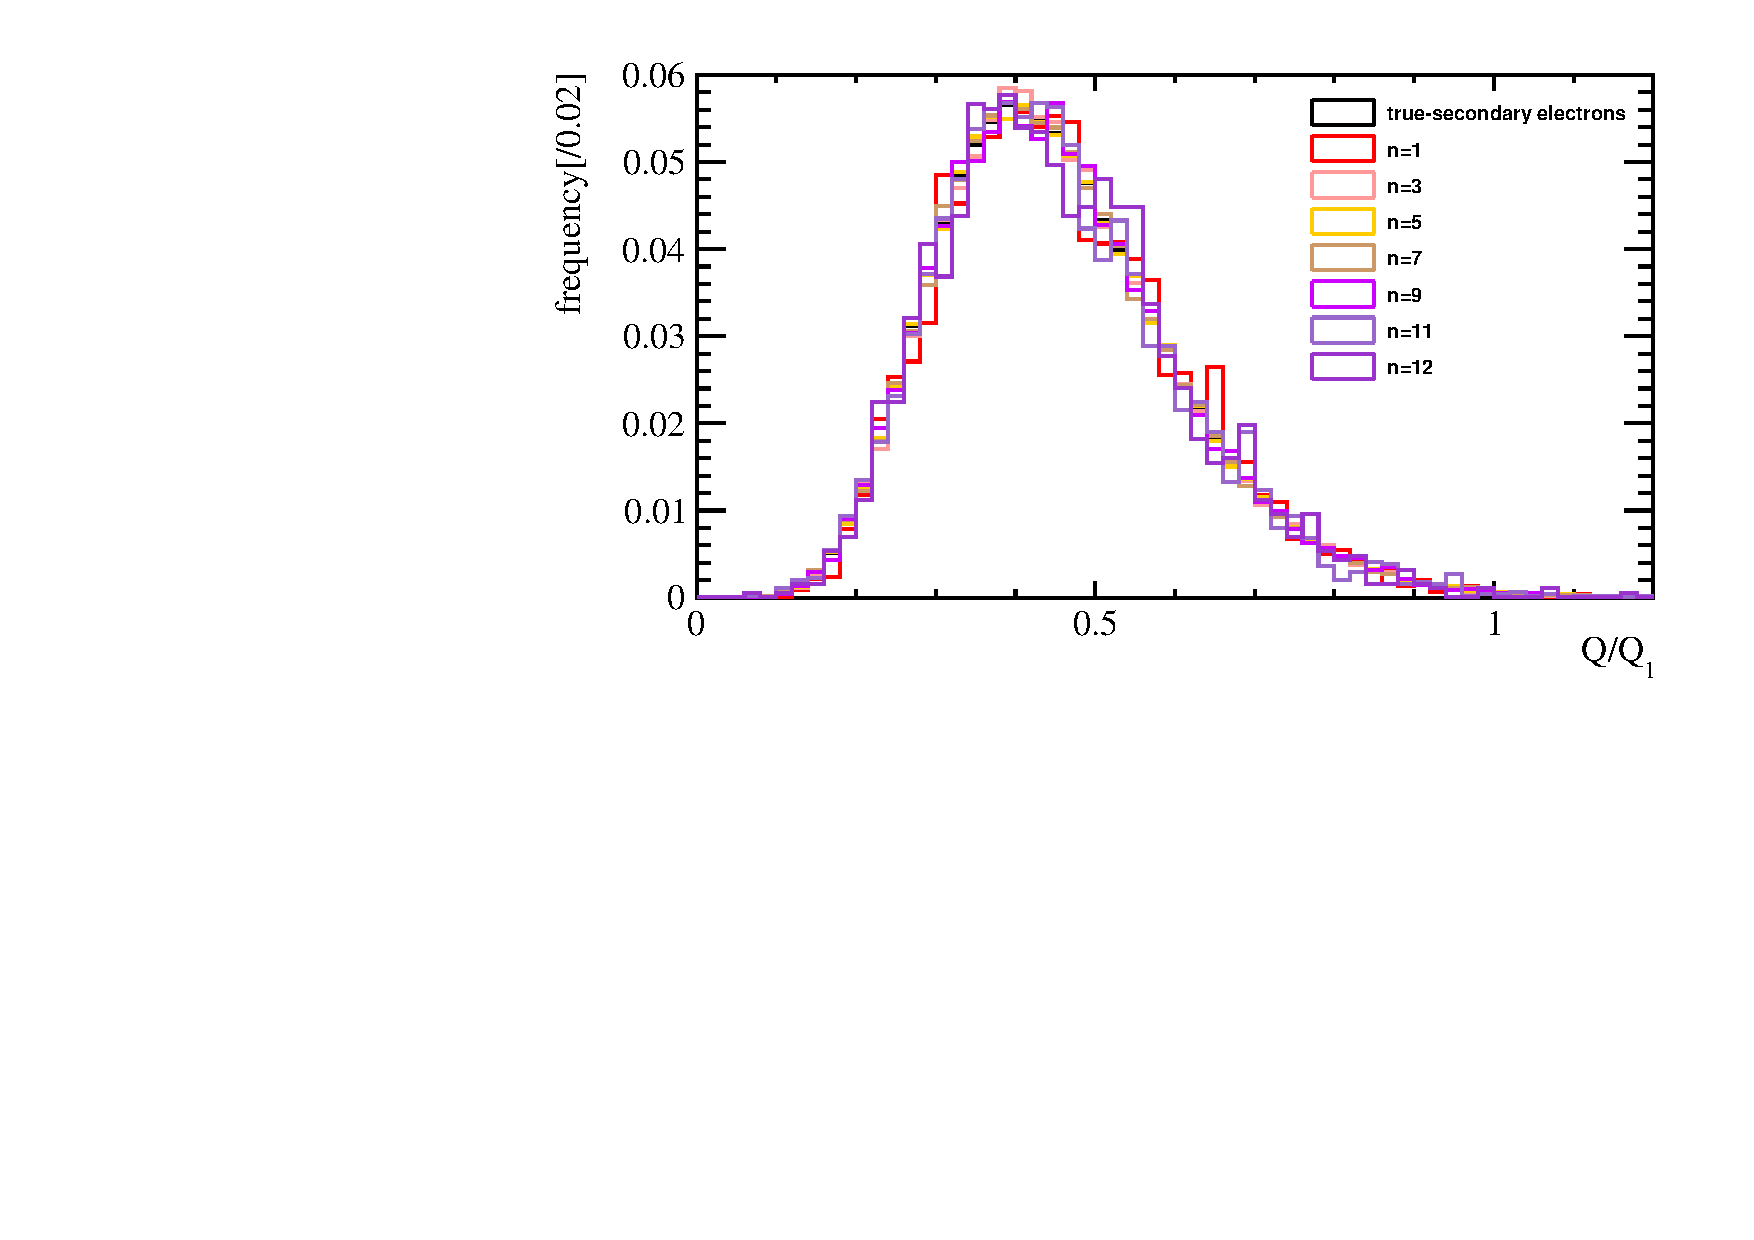
\includegraphics[width=\linewidth]{pic/single_pecharge.pdf}
        \caption{}
        \label{fig:single_pe}
    \end{subfigure}
    \hfill
    \begin{subfigure}{0.45\textwidth}
        \centering
        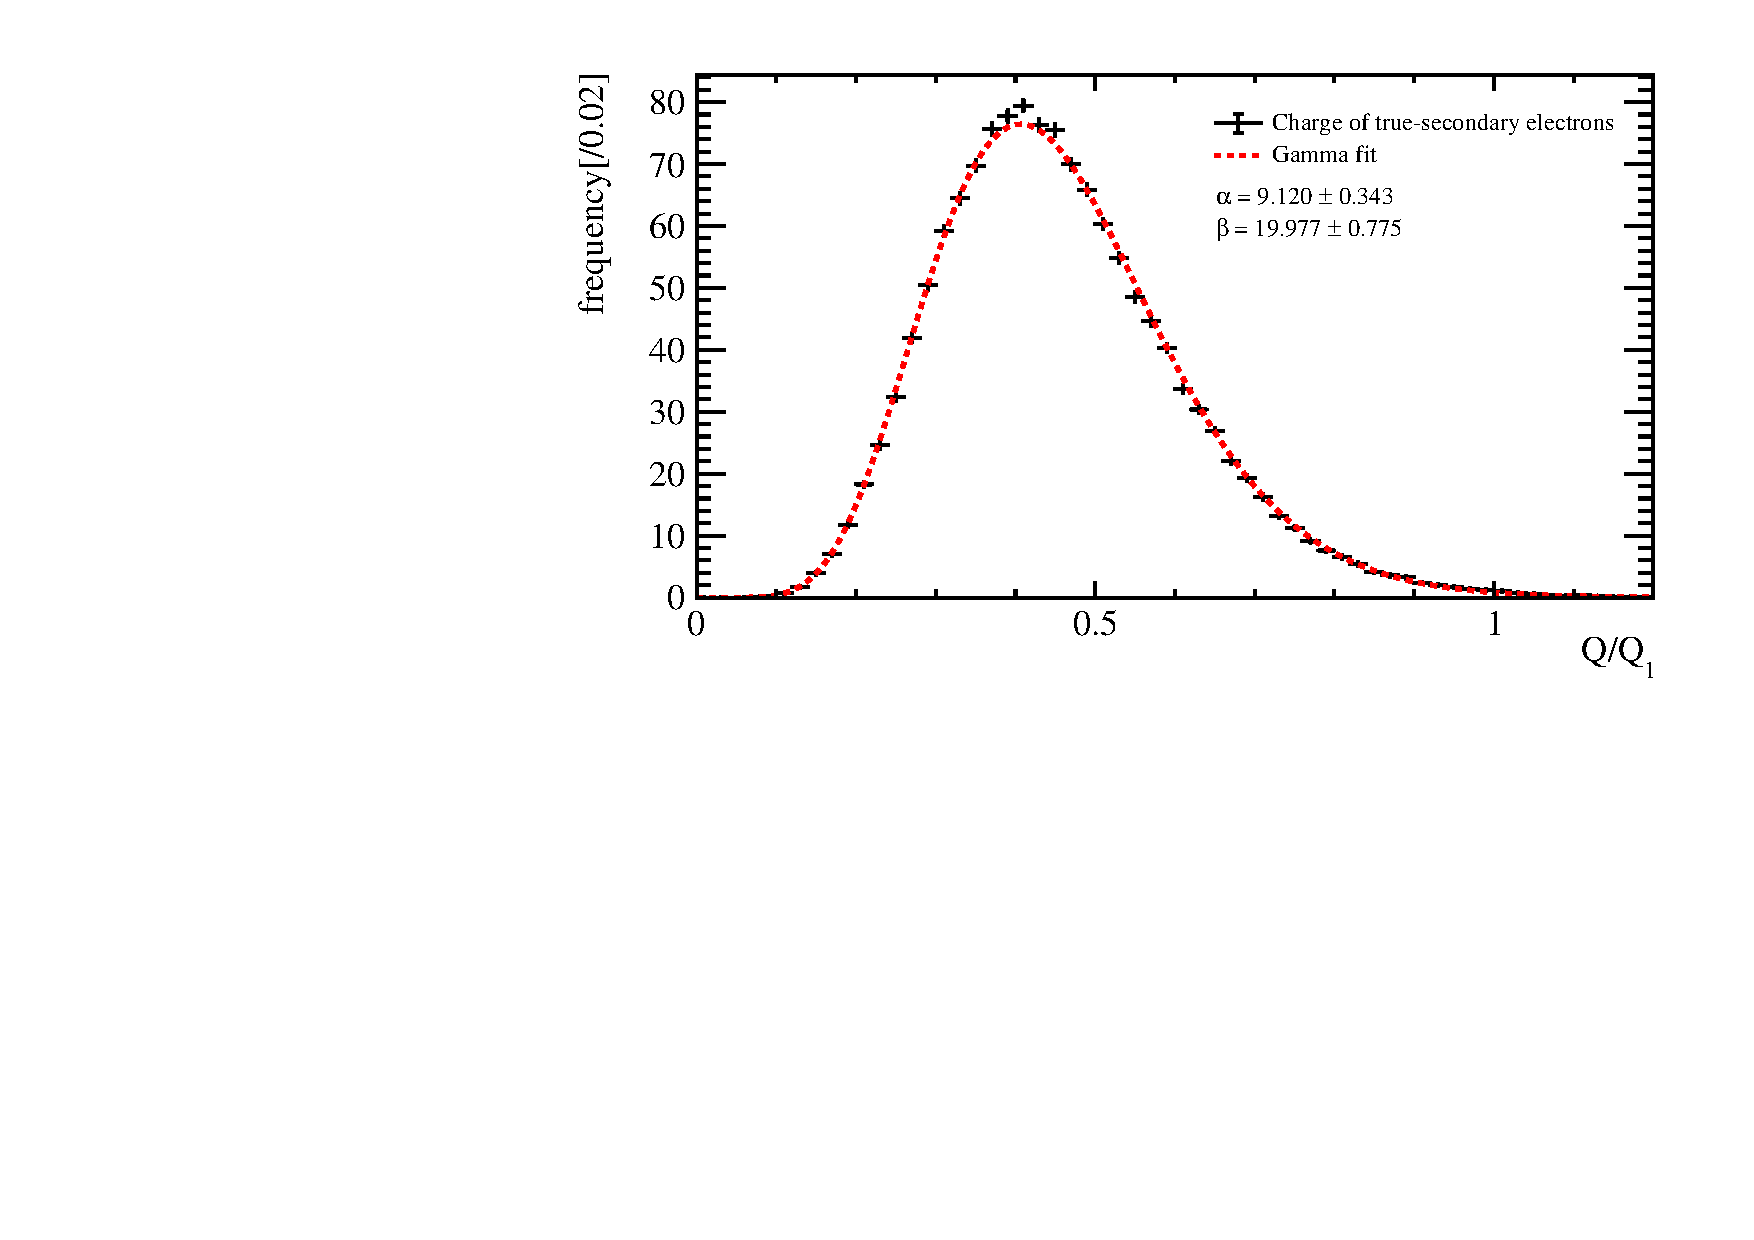
\includegraphics[width=\linewidth]{pic/singlepefit.pdf}
        \caption{}
        \label{fig:single_fit}
    \end{subfigure}
    \caption{The charge response distribution of single true-secondary electron when $n$ is different.
        The plot~\subref{fig:single_pe} shows that all the charges of true-secondary electrons follow the same distribution
        although $n$ is different.
        The plot~\subref{fig:single_fit} shows that the fitting of Gamma distribution on the charge response of single true-secondary electrons
        achieves sufficient goodness.}
    \label{fig:singlepe}
\end{figure}
$Q_{\mathrm{ts}}$ can be written as a sum of the same $n$ Gamma distributions as Eq.\eqref{eq:qts},
\begin{equation}
    \label{eq:qts}
    \begin{aligned}
         & Q_{\mathrm{ts}}=\sum_{n=0}^{\infty}\sum_{i=0}^{n}Q_{\mathrm{i}} \\
         & Q_{\mathrm{i}} \sim \varGamma(\alpha,\beta)                     \\
         & n \sim \mathrm{\pi}(\delta_{\mathrm{ts}})
    \end{aligned}
\end{equation}
which is a compound Poisson-Gamma distribution, belong to the Tweedie distribution~($\mathrm{Tw}_{\mathrm{t}}(\alpha,\beta)$)
when Tweedie power parameter $\mathrm{t}$ satisfies $1<\mathrm{t}<2$~\cite{Sen1997TheTO,1991Tweedie}.
The SER charge spectrum can be written as a Gamma-Tweedie mixture shown as Eq.~\eqref{eq:gTweedie}:
\begin{equation}
    \label{eq:gTweedie}
    \begin{aligned}
        Q_{\mathrm{MCP-PMT}} & = p_0\times Q_{\mathrm{peak}} + (1-p_0)Q_{\mathrm{ts}}                          \\
                             & Q_{\mathrm{peak}} \sim \varGamma(\alpha_{\mathrm{p}},\beta_{\mathrm{p}})        \\
                             & Q_{\mathrm{ts}} \sim \mathrm{Tw}_{\mathrm{t}}(\alpha,\beta),   1< \mathrm{t} <2
    \end{aligned}
\end{equation}


The MC calculation and chi-square test performed earlier in Sec.~\ref{sec:convolution} and \ref{subsec:chitest}
essentially constitute a joint fitting of the Gamma-Tweedie mixture.
This type of fitting is rather complex and impractical, requiring extensive computation.


